% ==============================================================
% P7 – Learning-Based Path Planning with ROS
% Final Project – Robotics and AI – IA2S Master – UPEC
% ==============================================================
\documentclass[aspectratio=169, 11pt]{beamer}

% ---------- Theme & UPEC Colors ----------
\usetheme{Madrid}
\usecolortheme{whale}

% UPEC brand colors: red + dark charcoal
\definecolor{upecred}{RGB}{206, 32, 41}
\definecolor{upecdark}{RGB}{35, 31, 32}
\definecolor{upecgray}{RGB}{100, 100, 100}
\definecolor{lightgray}{RGB}{245, 245, 245}
\definecolor{softblue}{RGB}{44, 82, 130}
\definecolor{softgreen}{RGB}{39, 124, 72}

\setbeamercolor{structure}{fg=upecred}
\setbeamercolor{palette primary}{bg=upecdark, fg=white}
\setbeamercolor{palette secondary}{bg=upecred, fg=white}
\setbeamercolor{palette tertiary}{bg=upecred!80!black, fg=white}
\setbeamercolor{palette quaternary}{bg=upecdark, fg=white}
\setbeamercolor{frametitle}{bg=upecdark, fg=white}
\setbeamercolor{title}{fg=upecdark}
\setbeamercolor{subtitle}{fg=upecred}
\setbeamercolor{block title}{bg=upecdark, fg=white}
\setbeamercolor{block body}{bg=lightgray}
\setbeamercolor{block title alerted}{bg=upecred, fg=white}
\setbeamercolor{block body alerted}{bg=upecred!8}
\setbeamercolor{block title example}{bg=softgreen, fg=white}
\setbeamercolor{block body example}{bg=softgreen!8}
\setbeamercolor{item}{fg=upecred}

% ---------- Packages ----------
\usepackage[utf8]{inputenc}
\usepackage[T1]{fontenc}
\usepackage{lmodern}
\usepackage{tikz}
\usetikzlibrary{shapes, arrows.meta, positioning, calc}
\usepackage{booktabs}
\usepackage{graphicx}
\usepackage{amsmath}
\usepackage{listings}
\usepackage{xcolor}
\usepackage{hyperref}

% ---------- Listings Style ----------
\lstset{
  basicstyle=\ttfamily\scriptsize,
  keywordstyle=\color{upecdark}\bfseries,
  commentstyle=\color{upecgray},
  stringstyle=\color{softgreen},
  backgroundcolor=\color{lightgray},
  frame=single,
  rulecolor=\color{gray!40},
  breaklines=true,
  showstringspaces=false,
}

% ---------- Title Info ----------
\title[P7 -- Learning-Based Path Planning with ROS]{%
  \textbf{Learning-Based Path Planning with ROS}}
\subtitle{AI-Based Navigation Strategy in Simulation}
\author[Benhamlaoui \& Brahimi]{%
  Benhamlaoui Abderrahmene Amar \and Brahimi Redha Wassim}
\institute[UPEC]{%
  Master IA2S -- Robotics and AI\\
  Universit\'{e} Paris-Est Cr\'{e}teil (UPEC)\\[0.3em]
  \textit{Supervisor:} Prof.\ Samer Mohammed}
\date{February 12, 2026}

% Logo in header
\logo{
\includegraphics[height=0.7cm]{figures/UPEC-logo.svg.png}}

% Remove navigation symbols
\setbeamertemplate{navigation symbols}{}

% Slide numbers in footer
\setbeamertemplate{footline}{%
  \leavevmode\hbox{%
    \begin{beamercolorbox}[wd=.33\paperwidth, ht=2.5ex, dp=1ex, center]
      {palette primary}%
      \usebeamerfont{author in head/foot}\insertshortauthor
    \end{beamercolorbox}%
    \begin{beamercolorbox}[wd=.44\paperwidth, ht=2.5ex, dp=1ex, center]
      {palette secondary}%
      \usebeamerfont{title in head/foot}\insertshorttitle
    \end{beamercolorbox}%
    \begin{beamercolorbox}[wd=.23\paperwidth, ht=2.5ex, dp=1ex, right]
      {palette tertiary}%
      \insertframenumber{} / \inserttotalframenumber\hspace*{2ex}
    \end{beamercolorbox}%
  }\vskip0pt}

% ==============================================================
\begin{document}

% -------------------- TITLE SLIDE --------------------
{
\setbeamertemplate{footline}{}
\begin{frame}
  \begin{columns}[c]
    \begin{column}{0.20\textwidth}
      \centering
      
\includegraphics[width=\linewidth]{figures/UPEC-logo.svg.png}
    \end{column}
    \begin{column}{0.78\textwidth}
      \vspace{0.3cm}
      {\large\color{upecgray} Master IA2S -- Robotics and AI}\\[0.1cm]
      {\small\color{upecgray} Universit\'{e} Paris-Est Cr\'{e}teil}\\[0.6cm]
      {\LARGE\bfseries\color{upecdark} Learning-Based Path Planning with ROS}\\[0.3cm]
      {\large\color{upecred} AI-Based Navigation Strategy in Simulation}\\[0.6cm]
      {\normalsize
        \textbf{Authors:} Benhamlaoui Abderrahmene Amar
        \& Brahimi Redha Wassim\\[0.2cm]
        \textbf{Supervisor:} Prof.\ Samer Mohammed\\[0.2cm]
        \textbf{Date:} February 12, 2026}
    \end{column}
  \end{columns}

  \vspace{0.5cm}
  \begin{center}
    \textcolor{upecred}{\rule{0.7\textwidth}{1.5pt}}\\[0.2cm]
    {\small\color{upecgray} Final Project -- P7: Learning-Based Path Planning}
  \end{center}
\end{frame}
}

% -------------------- OUTLINE --------------------
\begin{frame}{Outline}
  \tableofcontents
\end{frame}

% ============================================================
\section{Introduction}
% ============================================================

% -------------------- SLIDE: Context --------------------
\begin{frame}{Context and Motivation}

  \begin{columns}[T]
    \begin{column}{0.55\textwidth}
      \textbf{The challenge:} Make a robot navigate on its own,
      avoiding obstacles, \textbf{without a pre-built map}.

      \vspace{0.4em}
      \textbf{Old way} (traditional methods):
      \begin{itemize}
        \item Need a \textbf{map} of the environment first
        \item Many separate modules to configure by hand
        \item Doesn't adapt well to new situations
      \end{itemize}

      \vspace{0.4em}
      \textbf{Our way} (AI / learning-based):
      \begin{itemize}
        \item Robot \textbf{learns by itself} through practice
        \item Uses only its \textbf{laser sensor} (no map needed)
        \item \textbf{Adapts} to new environments automatically
      \end{itemize}
    \end{column}

    \begin{column}{0.42\textwidth}
      \centering
      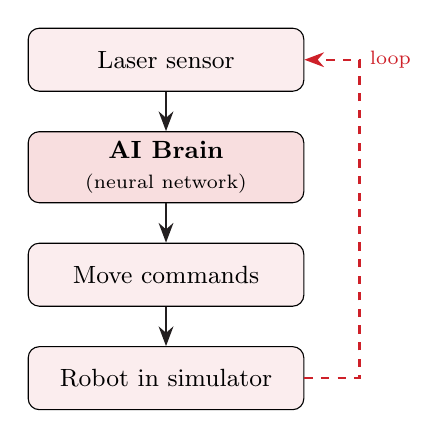
\begin{tikzpicture}[
        box/.style={draw, rounded corners, fill=upecred!8,
                     minimum width=3.5cm, minimum height=0.8cm,
                     align=center, font=\small},
        arr/.style={-{Stealth[length=2.5mm]}, thick, upecdark}
      ]
        \node[box] (sense) {Laser sensor};
        \node[box, below=0.5cm of sense, fill=upecred!15]
          (ai) {\textbf{AI Brain}\\{\scriptsize(neural network)}};
        \node[box, below=0.5cm of ai] (act) {Move commands};
        \node[box, below=0.5cm of act] (env) {Robot in simulator};
        \draw[arr] (sense) -- (ai);
        \draw[arr] (ai) -- (act);
        \draw[arr] (act) -- (env);
        \draw[arr, dashed, upecred] (env.east) -- ++(0.7,0)
              |- (sense.east) node[midway, right, font=\scriptsize,
              upecred] {loop};
      \end{tikzpicture}
    \end{column}
  \end{columns}
\end{frame}

% -------------------- SLIDE: Project Goal --------------------
\begin{frame}{Project Objective}

  \begin{alertblock}{Assignment (P7)}
    Integrate a learning-based navigation policy into ROS to control
    a robot in simulation. Focus on observing how the AI model influences
    path planning and obstacle avoidance.
  \end{alertblock}

  \vspace{0.5em}

  \begin{columns}[T]
    \begin{column}{0.32\textwidth}
      \centering
      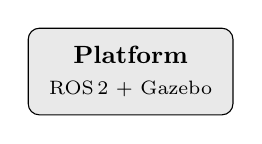
\begin{tikzpicture}
        \node[draw, rounded corners, fill=upecdark!10,
              minimum width=2.6cm, minimum height=1.1cm,
              align=center, font=\small]
              {\textbf{Platform}\\{\scriptsize ROS\,2 + Gazebo}};
      \end{tikzpicture}
    \end{column}
    \begin{column}{0.32\textwidth}
      \centering
      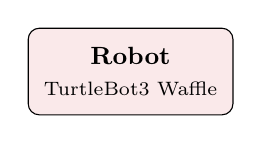
\begin{tikzpicture}
        \node[draw, rounded corners, fill=upecred!10,
              minimum width=2.6cm, minimum height=1.1cm,
              align=center, font=\small]
              {\textbf{Robot}\\{\scriptsize TurtleBot3 Waffle}};
      \end{tikzpicture}
    \end{column}
    \begin{column}{0.32\textwidth}
      \centering
      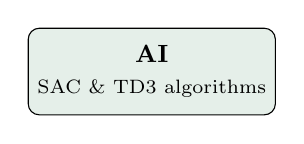
\begin{tikzpicture}
        \node[draw, rounded corners, fill=softgreen!12,
              minimum width=2.6cm, minimum height=1.1cm,
              align=center, font=\small]
              {\textbf{AI}\\{\scriptsize SAC \& TD3 algorithms}};
      \end{tikzpicture}
    \end{column}
  \end{columns}

  \vspace{0.5em}

  \begin{block}{What we show in this project}
    \begin{itemize}
      \item How an AI agent is plugged into a ROS\,2 robot system
      \item How it learns to navigate using only sensor data
      \item How we track its progress (rewards, collisions, successes)
    \end{itemize}
  \end{block}
\end{frame}

% ============================================================
\section{How the AI Works}
% ============================================================

% -------------------- SLIDE: What is RL --------------------
\begin{frame}{Reinforcement Learning -- The Big Idea}

  \textbf{Reinforcement Learning (RL)} = the robot learns by
  \textbf{trial and error}, like training a pet.

  \vspace{0.4em}

  \begin{center}
  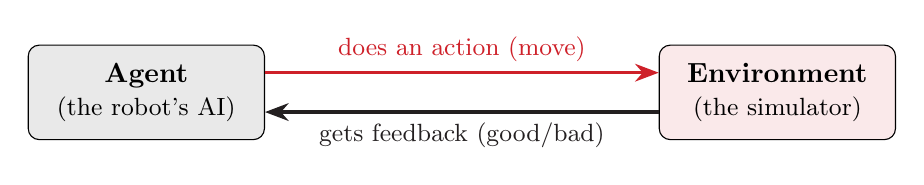
\begin{tikzpicture}[
    arr/.style={-{Stealth[length=3mm]}, very thick}
  ]
    \node[draw, rounded corners, fill=upecdark!10,
          minimum width=3cm, minimum height=1.2cm,
          align=center, font=\normalsize] (agent)
          {\textbf{Agent}\\{\small(the robot's AI)}};
    \node[draw, rounded corners, fill=upecred!10,
          minimum width=3cm, minimum height=1.2cm,
          align=center, font=\normalsize, right=5cm of agent] (envir)
      {\textbf{Environment}\\{\small(the simulator)}};

    \draw[arr, upecred]
      ([yshift=0.25cm]agent.east) -- node[above, font=\small]
      {does an action (move)} ([yshift=0.25cm]envir.west);
    \draw[arr, upecdark]
      ([yshift=-0.25cm]envir.west) -- node[below, font=\small]
      {gets feedback (good/bad)} ([yshift=-0.25cm]agent.east);
  \end{tikzpicture}
  \end{center}

  \vspace{0.3em}

  \begin{columns}[T]
    \begin{column}{0.48\textwidth}
      \begin{block}{The learning cycle}
        \begin{enumerate}\small
          \item Robot \textbf{looks} at its surroundings
          \item Robot \textbf{decides} how to move
          \item Gets a \textbf{score} (reward or penalty)
          \item \textbf{Improves} its strategy over time
        \end{enumerate}
      \end{block}
    \end{column}
    \begin{column}{0.48\textwidth}
      \begin{exampleblock}{Simple analogy}
        Like teaching a dog:\vspace{-0.2em}
        \begin{itemize}\small
          \item Dog tries something (move somewhere)
          \item Gets a treat (+) or a ``no!'' ($-$)
          \item Over time, learns the right behavior
        \end{itemize}
      \end{exampleblock}
    \end{column}
  \end{columns}
\end{frame}

% -------------------- SLIDE: Deep RL --------------------
\begin{frame}{Why ``Deep'' Reinforcement Learning?}

  \begin{columns}[T]
    \begin{column}{0.48\textwidth}
      The robot's world is complex -- it receives
      \textbf{25 numbers} describing its surroundings every step.

      \vspace{0.4em}
      A simple lookup table can't handle this.
      So we use a \textbf{neural network} (a brain-like program)
      that can learn patterns from experience.

      \vspace{0.4em}
      \textbf{Deep RL} = Reinforcement Learning
      + Neural Networks

      \vspace{0.3em}
      \begin{itemize}
        \item The network takes \textbf{25 inputs}
              (what the robot sees)
        \item Processes them through hidden layers
        \item Outputs \textbf{2 values}
              (speed + turn direction)
      \end{itemize}
    \end{column}

    \begin{column}{0.48\textwidth}
      \centering
      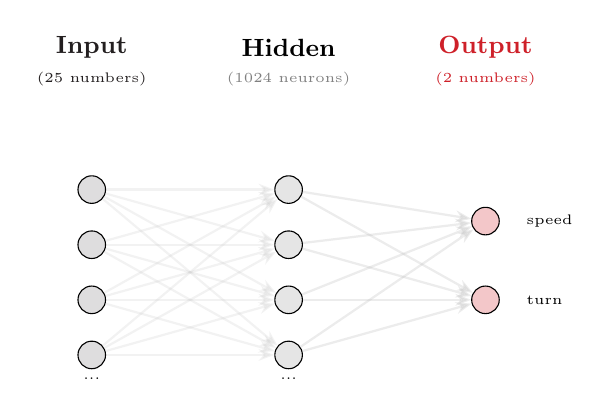
\begin{tikzpicture}[
        arr/.style={-{Stealth[length=2mm]}, thick, gray!50}
      ]
        % Input
        \node[font=\small\bfseries, upecdark] at (-1.5, 2.8) {Input};
        \node[font=\tiny, upecdark] at (-1.5, 2.4) {(25 numbers)};
        \foreach \i in {1,...,4}{
          \node[circle, draw, fill=upecdark!15, minimum size=0.35cm,
                inner sep=0pt] (in\i) at (-1.5, 1.7 - \i*0.7) {};
        }
        \node[font=\tiny] at (-1.5, -1.4) {...};

        % Hidden
        \node[font=\small\bfseries] at (1, 2.8) {Hidden};
        \node[font=\tiny, gray] at (1, 2.4) {(1024 neurons)};
        \foreach \i in {1,...,4}{
          \node[circle, draw, fill=gray!20, minimum size=0.35cm,
                inner sep=0pt] (h\i) at (1, 1.7 - \i*0.7) {};
        }
        \node[font=\tiny] at (1, -1.4) {...};

        % Output
        \node[font=\small\bfseries, upecred] at (3.5, 2.8) {Output};
        \node[font=\tiny, upecred] at (3.5, 2.4) {(2 numbers)};
        \node[circle, draw, fill=upecred!25, minimum size=0.35cm,
              inner sep=0pt] (out1) at (3.5, 0.6) {};
        \node[circle, draw, fill=upecred!25, minimum size=0.35cm,
              inner sep=0pt] (out2) at (3.5, -0.4) {};
        \node[font=\tiny, right] at (3.9, 0.6) {speed};
        \node[font=\tiny, right] at (3.9, -0.4) {turn};

        % Connections
        \foreach \i in {1,...,4}{
          \foreach \j in {1,...,4}{
            \draw[arr, opacity=0.2] (in\i) -- (h\j);
          }
          \draw[arr, opacity=0.3] (h\i) -- (out1);
          \draw[arr, opacity=0.3] (h\i) -- (out2);
        }
      \end{tikzpicture}

      \vspace{0.3em}
      {\scriptsize\color{upecgray}
        The network has $\sim$2 million adjustable parameters\\
        that are tuned during training.}
    \end{column}
  \end{columns}
\end{frame}

% ============================================================
\section{Platform \& Setup}
% ============================================================

% -------------------- SLIDE: Tools --------------------
\begin{frame}{Tools We Used}

  \begin{center}
  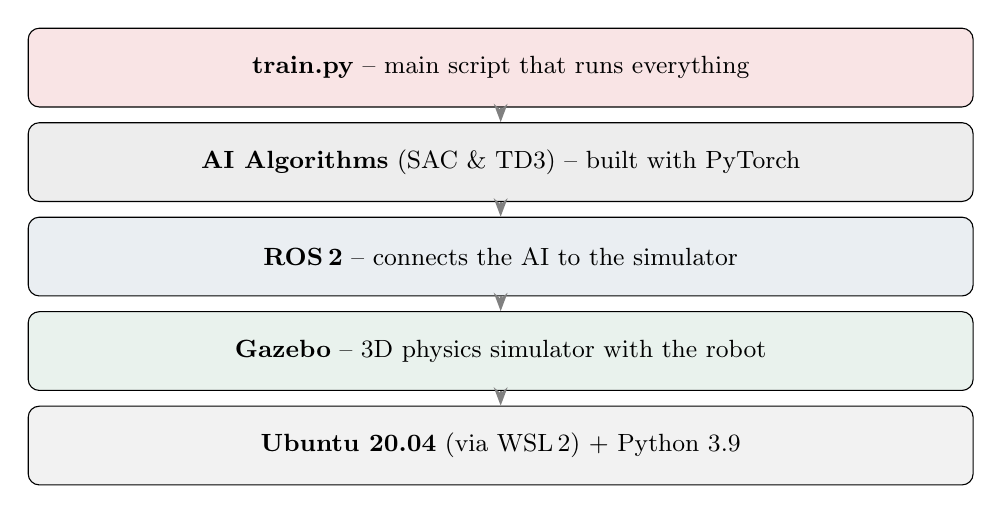
\begin{tikzpicture}[
    layer/.style={draw, rounded corners, minimum width=12cm,
                  minimum height=1.0cm, align=center, font=\small},
    arr/.style={-{Stealth}, thick, gray}
  ]
    \node[layer, fill=upecred!12] (app) at (0, 3.6)
      {\textbf{train.py} -- main script that runs everything};
    \node[layer, fill=upecdark!8] (drl) at (0, 2.4)
      {\textbf{AI Algorithms} (SAC \& TD3) -- built with PyTorch};
    \node[layer, fill=softblue!10] (ros) at (0, 1.2)
      {\textbf{ROS\,2} -- connects the AI to the simulator};
    \node[layer, fill=softgreen!10] (gz) at (0, 0)
      {\textbf{Gazebo} -- 3D physics simulator with the robot};
    \node[layer, fill=gray!10] (os) at (0, -1.2)
      {\textbf{Ubuntu 20.04} (via WSL\,2) + Python 3.9};

    \draw[arr] (app) -- (drl);
    \draw[arr] (drl) -- (ros);
    \draw[arr] (ros) -- (gz);
    \draw[arr] (gz) -- (os);
  \end{tikzpicture}
  \end{center}

  \vspace{0.3em}
  \begin{center}
    {\small\color{upecgray}
    Each layer talks to the one below it -- clean and modular.}
  \end{center}
\end{frame}

% -------------------- SLIDE: Simulation --------------------
\begin{frame}{The Simulated World}

  \begin{columns}[T]
    \begin{column}{0.50\textwidth}
      \textbf{What's inside the simulator:}
      \begin{itemize}
        \item A \textbf{10m $\times$ 10m} walled arena
        \item \textbf{8 obstacles} (4 fixed + 4 random)
        \item A \textbf{TurtleBot3} robot with a laser scanner
        \item A \textbf{goal point} that moves each round
      \end{itemize}

      \vspace{0.5em}
      \textbf{How it runs:}
      \begin{itemize}
        \item The simulator pauses while the AI thinks
        \item AI decides, simulator advances 0.1 seconds
        \item This repeats until the robot reaches the
              goal or crashes
      \end{itemize}
    \end{column}

    \begin{column}{0.46\textwidth}
      \centering
      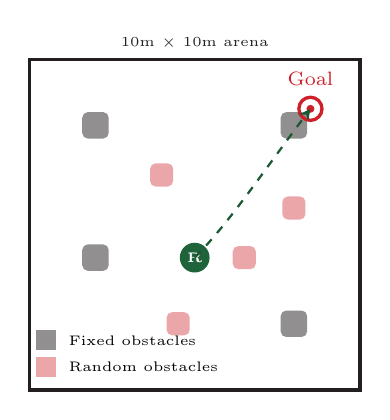
\begin{tikzpicture}[scale=0.42]
        % Arena
        \draw[very thick, upecdark] (-5,-5) rectangle (5,5);
        \node[font=\tiny, upecdark] at (0, 5.5) {10m $\times$ 10m arena};

        % Fixed obstacles (dark)
        \foreach \x/\y in {-3/3, 3/-3, -3/-1, 3/3}{
          \fill[upecdark!50, rounded corners=2pt]
            (\x-0.4, \y-0.4) rectangle (\x+0.4, \y+0.4);
        }
        % Random obstacles (red)
        \foreach \x/\y in {-1/1.5, 1.5/-1, -0.5/-3, 3/0.5}{
          \fill[upecred!40, rounded corners=2pt]
            (\x-0.35, \y-0.35) rectangle (\x+0.35, \y+0.35);
        }

        % Robot
        \fill[softgreen!80!black] (0,-1) circle (0.45);
        \node[font=\tiny\bfseries, white] at (0,-1) {R};

        % Goal
        \draw[upecred, very thick] (3.5, 3.5) circle (0.35);
        \fill[upecred] (3.5, 3.5) circle (0.12);
        \node[font=\scriptsize, above, upecred] at (3.5, 3.9) {Goal};

        % Path
        \draw[dashed, thick, softgreen!70!black, ->, >=stealth]
          (0,-1) .. controls (1,0) and (2,1.5) .. (3.5,3.5);

        % Legend
        \fill[upecdark!50] (-4.8, -3.8) rectangle (-4.2, -3.2);
        \node[font=\tiny, right] at (-4.1, -3.5) {Fixed obstacles};
        \fill[upecred!40] (-4.8, -4.6) rectangle (-4.2, -4.0);
        \node[font=\tiny, right] at (-4.1, -4.3) {Random obstacles};
      \end{tikzpicture}
    \end{column}
  \end{columns}
\end{frame}

% -------------------- SLIDE: ROS2 --------------------
\begin{frame}{How the Pieces Talk (ROS\,2)}

  \textbf{ROS\,2} is the ``postman'' that delivers messages between
  the simulator and the AI.

  \vspace{0.3em}

  \begin{center}
  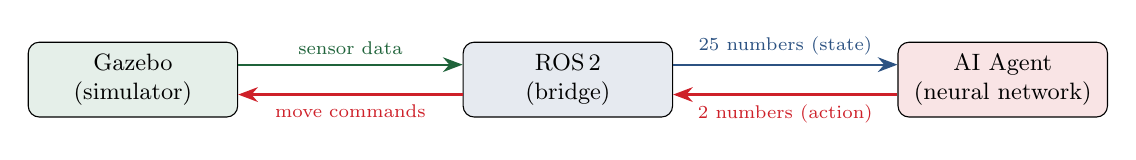
\begin{tikzpicture}[
    arr/.style={-{Stealth[length=2.5mm]}, thick},
    scale=0.95, transform shape
  ]
    \node[draw, rounded corners, fill=softgreen!12,
          minimum width=2.8cm, minimum height=1.0cm,
          align=center, font=\small] (gazebo) {Gazebo\\(simulator)};
    \node[draw, rounded corners, fill=softblue!12,
          minimum width=2.8cm, minimum height=1.0cm,
          align=center, font=\small, right=3cm of gazebo]
          (bridge) {ROS\,2\\(bridge)};
    \node[draw, rounded corners, fill=upecred!12,
          minimum width=2.8cm, minimum height=1.0cm,
          align=center, font=\small, right=3cm of bridge]
          (ai) {AI Agent\\(neural network)};

    \draw[arr, softgreen!80!black] ([yshift=0.2cm]gazebo.east) --
      node[above, font=\scriptsize]{sensor data}
      ([yshift=0.2cm]bridge.west);
    \draw[arr, softblue] ([yshift=0.2cm]bridge.east) --
      node[above, font=\scriptsize]{25 numbers (state)}
      ([yshift=0.2cm]ai.west);
    \draw[arr, upecred] ([yshift=-0.2cm]ai.west) --
      node[below, font=\scriptsize]{2 numbers (action)}
      ([yshift=-0.2cm]bridge.east);
    \draw[arr, upecred] ([yshift=-0.2cm]bridge.west) --
      node[below, font=\scriptsize]{move commands}
      ([yshift=-0.2cm]gazebo.east);
  \end{tikzpicture}
  \end{center}

  \vspace{0.4em}

  \begin{center}
  \small
  \renewcommand{\arraystretch}{1.15}
  \begin{tabular}{lll}
    \toprule
    \textbf{Message} & \textbf{Direction} & \textbf{What it carries}\\
    \midrule
    \texttt{/scan} & Simulator $\rightarrow$ AI &
      Laser distances (what's around the robot)\\
    \texttt{/odom} & Simulator $\rightarrow$ AI &
      Robot's position and orientation\\
    \texttt{/cmd\_vel} & AI $\rightarrow$ Simulator &
      Speed and turn commands\\
    \texttt{/reset\_world} & AI $\rightarrow$ Simulator &
      Reset the world for a new round\\
    \bottomrule
  \end{tabular}
  \end{center}
\end{frame}

% ============================================================
\section{What the Robot Sees and Does}
% ============================================================

% -------------------- SLIDE: State --------------------
\begin{frame}{What the Robot ``Sees'' -- 25 Numbers}

  Every 0.1 seconds, the AI receives \textbf{25 numbers}:

  \vspace{0.4em}

  \begin{center}
  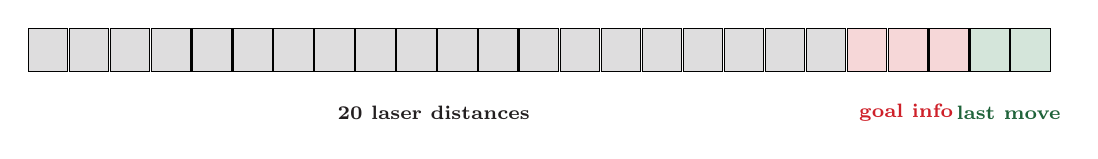
\begin{tikzpicture}
    % Laser bins
    \foreach \i in {0,...,19}{
      \node[draw, minimum width=0.5cm, minimum height=0.55cm,
            fill=upecdark!15, font=\tiny] at (\i*0.52, 0) {};
    }
    % Goal info
    \foreach \i in {20,21,22}{
      \pgfmathsetmacro{\pos}{\i*0.52}
      \node[draw, minimum width=0.5cm, minimum height=0.55cm,
            fill=upecred!18, font=\tiny] at (\pos, 0) {};
    }
    % Prev actions
    \foreach \i in {23,24}{
      \pgfmathsetmacro{\pos}{\i*0.52}
      \node[draw, minimum width=0.5cm, minimum height=0.55cm,
            fill=softgreen!20, font=\tiny] at (\pos, 0) {};
    }

    % Labels
    \node[font=\scriptsize\bfseries, upecdark] at (4.9, -0.8)
      {20 laser distances};
    \node[font=\scriptsize\bfseries, upecred] at (10.9, -0.8)
      {goal info};
    \node[font=\scriptsize\bfseries, softgreen!80!black] at (12.2, -0.8)
      {last move};
  \end{tikzpicture}
  \end{center}

  \vspace{0.4em}

  \begin{columns}[T]
    \begin{column}{0.32\textwidth}
      \textbf{\color{upecdark}Laser distances [0--19]}\\[0.2em]
      \small
      The 360-degree laser is split into \textbf{20 zones}.
      Each gives the closest obstacle distance.\\[0.2em]
      {\scriptsize Tells the robot: \textit{``What's around me?''}}
    \end{column}
    \begin{column}{0.32\textwidth}
      \textbf{\color{upecred}Goal info [20--22]}\\[0.2em]
      \small
      How \textbf{far} is the goal, and in which
      \textbf{direction} (as cos/sin angles).\\[0.2em]
      {\scriptsize Tells the robot: \textit{``Where should I go?''}}
    \end{column}
    \begin{column}{0.32\textwidth}
      \textbf{\color{softgreen!80!black}Last move [23--24]}\\[0.2em]
      \small
      The \textbf{previous speed} and \textbf{turn}
      the robot did.\\[0.2em]
      {\scriptsize Helps produce \textit{smoother movement}.}
    \end{column}
  \end{columns}
\end{frame}

% -------------------- SLIDE: Action --------------------
\begin{frame}{What the Robot ``Does'' -- 2 Numbers}

  The AI outputs \textbf{2 numbers} that control the robot:

  \vspace{0.6em}

  \begin{center}
  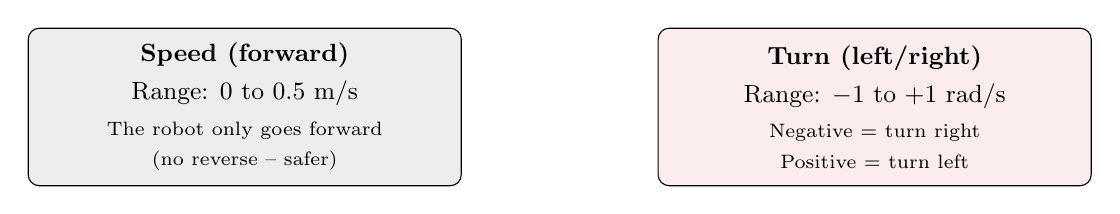
\begin{tikzpicture}
    \node[draw, rounded corners, fill=upecdark!8,
          minimum width=5.5cm, minimum height=2cm,
          align=center, font=\small] (lin) at (-4, 0) {
      \textbf{Speed (forward)}\\[0.3em]
      Range: 0 to 0.5 m/s\\[0.2em]
      {\scriptsize The robot only goes forward}\\
      {\scriptsize (no reverse -- safer)}
    };
    \node[draw, rounded corners, fill=upecred!8,
          minimum width=5.5cm, minimum height=2cm,
          align=center, font=\small] (ang) at (4, 0) {
      \textbf{Turn (left/right)}\\[0.3em]
      Range: $-1$ to $+1$ rad/s\\[0.2em]
      {\scriptsize Negative = turn right}\\
      {\scriptsize Positive = turn left}
    };
  \end{tikzpicture}
  \end{center}

  \vspace{0.5em}

  \begin{block}{Why continuous actions matter}
    The robot can choose \textbf{any speed and turn angle} in the range,
    not just ``go left'' or ``go right.'' This produces
    \textbf{smooth, natural paths}.
  \end{block}
\end{frame}

% -------------------- SLIDE: Reward --------------------
\begin{frame}{The Scoring System (Reward Function)}

  The AI learns by getting \textbf{scores} after every action:

  \vspace{0.3em}

  \begin{center}
  \renewcommand{\arraystretch}{1.3}
  \begin{tabular}{lrl}
    \toprule
    \textbf{What happens} & \textbf{Score} & \textbf{Why}\\
    \midrule
    Reaches the goal & \textbf{+100} & Big reward for success\\
    Hits an obstacle & \textbf{$-$100} & Big penalty for crashing\\
    Moves forward & \textbf{+small} & Encourage progress\\
    Spins in place & \textbf{$-$small} & Discourage wasting time\\
    Gets too close to obstacle & \textbf{$-$small} & Keep safe distance\\
    \bottomrule
  \end{tabular}
  \end{center}

  \vspace{0.4em}

  \begin{exampleblock}{How the robot improves}
    Over thousands of rounds, the robot learns to
    \textbf{maximize its total score} -- which means reaching goals
    while avoiding obstacles. It's like playing a video game and
    trying to get the highest score!
  \end{exampleblock}
\end{frame}

% ============================================================
\section{The AI Algorithms}
% ============================================================

% -------------------- SLIDE: SAC --------------------
\begin{frame}{SAC -- The Main Algorithm}

  \textbf{SAC} (Soft Actor-Critic) is the primary AI algorithm used.
  Think of it as \textbf{two cooperating teammates}:

  \vspace{0.4em}

  \begin{center}
  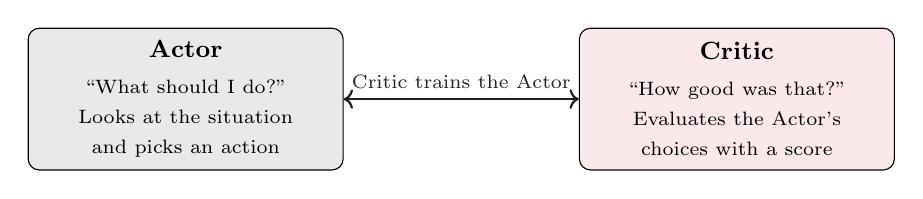
\begin{tikzpicture}[
    arr/.style={-{Stealth[length=2.5mm]}, thick}
  ]
    \node[draw, rounded corners, fill=upecdark!10,
          minimum width=4cm, minimum height=1.8cm,
          align=center, font=\small] (actor) at (-3.5, 0) {
      \textbf{Actor}\\[0.2em]
      \scriptsize ``What should I do?''\\
      \scriptsize Looks at the situation\\
      \scriptsize and picks an action
    };
    \node[draw, rounded corners, fill=upecred!10,
          minimum width=4cm, minimum height=1.8cm,
          align=center, font=\small] (critic) at (3.5, 0) {
      \textbf{Critic}\\[0.2em]
      \scriptsize ``How good was that?''\\
      \scriptsize Evaluates the Actor's\\
      \scriptsize choices with a score
    };
    \draw[arr, upecdark, <->] (actor) -- node[above, font=\scriptsize]
      {Critic trains the Actor} (critic);
  \end{tikzpicture}
  \end{center}

  \vspace{0.3em}

  \textbf{What makes SAC special:}
  \begin{enumerate}\small
    \item \textbf{Encourages exploration}: the robot is rewarded for
          \textit{trying different things}, so it doesn't get stuck
          in one strategy
    \item \textbf{Two critics}: uses 2 separate critics and takes the
          lower score -- prevents the AI from being overconfident
    \item \textbf{Self-adjusting}: automatically balances between
          exploring and using what it already knows
  \end{enumerate}
\end{frame}

% -------------------- SLIDE: TD3 --------------------
\begin{frame}{TD3 -- The Alternative Algorithm}

  \textbf{TD3} (Twin Delayed DDPG) is the second algorithm available
  in the project.

  \vspace{0.4em}

  \begin{columns}[T]
    \begin{column}{0.48\textwidth}
      \begin{block}{How TD3 is different from SAC}
        \begin{itemize}\small
          \item \textbf{Always picks the same move} for a given
                situation (deterministic)
          \item Explores by adding \textbf{random noise}
                to its actions during training
          \item Updates the Actor \textbf{less frequently}
                for more stable learning
        \end{itemize}
      \end{block}
    \end{column}

    \begin{column}{0.48\textwidth}
      \begin{alertblock}{SAC vs.\ TD3}
        \renewcommand{\arraystretch}{1.3}
        \small
        \begin{tabular}{lcc}
          & \textbf{SAC} & \textbf{TD3}\\
          \midrule
          Strategy & Random & Fixed\\
          Exploration & Built-in & Added noise\\
          Tuning & Automatic & Manual\\
        \end{tabular}
      \end{alertblock}

      \vspace{0.3em}
      {\small\color{upecgray}
        SAC usually works better for robot navigation
        because it explores more naturally.}
    \end{column}
  \end{columns}
\end{frame}

% ============================================================
\section{Training Process}
% ============================================================

% -------------------- SLIDE: Pipeline --------------------
\begin{frame}{How Training Works}

  \begin{columns}[T]
    \begin{column}{0.45\textwidth}
      \centering
      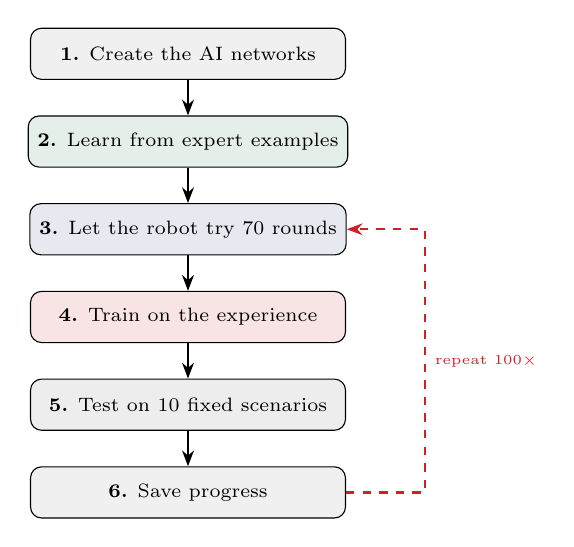
\begin{tikzpicture}[
        node distance=0.45cm,
        arr/.style={-{Stealth[length=2mm]}, thick},
        box/.style={draw, rounded corners, minimum width=4cm,
                    minimum height=0.65cm, align=center, font=\scriptsize}
      ]
        \node[box, fill=gray!12] (init) {\textbf{1.} Create the AI networks};
        \node[box, fill=softgreen!12, below=of init] (pre)
              {\textbf{2.} Learn from expert examples};
        \node[box, fill=softblue!12, below=of pre] (ep)
              {\textbf{3.} Let the robot try 70 rounds};
        \node[box, fill=upecred!12, below=of ep] (train)
              {\textbf{4.} Train on the experience};
        \node[box, fill=upecdark!8, below=of train] (eval)
              {\textbf{5.} Test on 10 fixed scenarios};
        \node[box, fill=gray!12, below=of eval] (log)
              {\textbf{6.} Save progress};

        \draw[arr] (init) -- (pre);
        \draw[arr] (pre) -- (ep);
        \draw[arr] (ep) -- (train);
        \draw[arr] (train) -- (eval);
        \draw[arr] (eval) -- (log);
        \draw[arr, dashed, upecred] (log.east) -- ++(1.0,0) |- (ep.east)
          node[pos=0.25, right, font=\tiny] {repeat 100$\times$};
      \end{tikzpicture}
    \end{column}

    \begin{column}{0.52\textwidth}
      \textbf{Memory bank (Replay Buffer):}
      \begin{itemize}\small
        \item Stores the last \textbf{5000 experiences}
        \item Each experience = what happened, what it did,
              what score it got
        \item Training picks random experiences to learn from
        \item This helps the AI learn from \textbf{past mistakes}
      \end{itemize}

      \vspace{0.3em}
      \textbf{Numbers:}
      \begin{itemize}\small
        \item 100 rounds of training (epochs)
        \item 70 episodes per round
        \item = \textbf{7,000 total episodes} of practice
        \item Each episode: up to 300 steps
      \end{itemize}

      \vspace{0.2em}
      {\small\color{upecgray}
        That's millions of decisions the robot makes during training!}
    \end{column}
  \end{columns}
\end{frame}

% -------------------- SLIDE: Pre-training --------------------
\begin{frame}{Getting a Head Start (Pre-training)}

  \begin{columns}[T]
    \begin{column}{0.55\textwidth}
      Instead of starting completely random, we give the AI
      a \textbf{head start} using recorded expert data.

      \vspace{0.4em}
      \textbf{How it works:}
      \begin{enumerate}\small
        \item An expert drove the robot and we \textbf{recorded}
              every move (saved in a file called \texttt{data.yml})
        \item The AI first \textbf{copies} the expert's behavior
              (50 training rounds)
        \item Then it continues learning on its own and
              \textbf{gets even better} than the expert
      \end{enumerate}

      \vspace{0.3em}
      \begin{alertblock}{Why this matters}
        \small Without pre-training: robot crashes randomly for hours.\\
        With pre-training: robot can navigate from the start!
      \end{alertblock}
    \end{column}

    \begin{column}{0.42\textwidth}
      \centering
      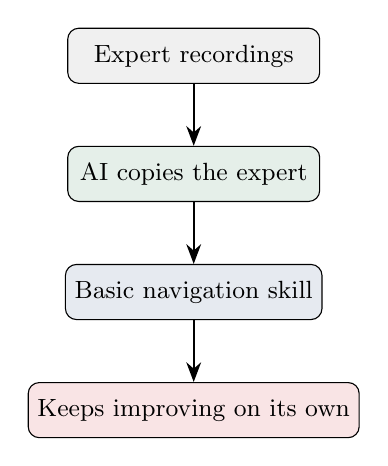
\begin{tikzpicture}[
        arr/.style={-{Stealth[length=2.5mm]}, thick},
        box/.style={draw, rounded corners, minimum width=3.2cm,
                    minimum height=0.7cm, align=center, font=\small}
      ]
        \node[box, fill=gray!12] (data) at (0, 2.5)
              {Expert recordings};
        \node[box, fill=softgreen!12] (copy) at (0, 1.0)
              {AI copies the expert};
        \node[box, fill=softblue!12] (good) at (0, -0.5)
              {Basic navigation skill};
        \node[box, fill=upecred!12] (online) at (0, -2.0)
              {Keeps improving on its own};

        \draw[arr] (data) -- (copy);
        \draw[arr] (copy) -- (good);
        \draw[arr] (good) -- (online);
      \end{tikzpicture}
    \end{column}
  \end{columns}
\end{frame}

% -------------------- SLIDE: Curriculum --------------------
\begin{frame}{Progressive Difficulty (Curriculum Learning)}

  The training starts \textbf{easy} and gets \textbf{harder} over time:

  \vspace{0.3em}

  \begin{columns}[T]
    \begin{column}{0.48\textwidth}
      \centering
      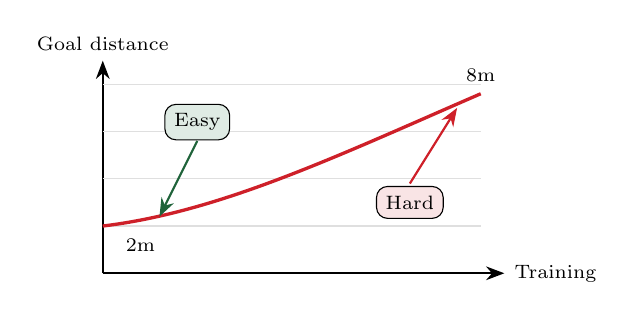
\begin{tikzpicture}[scale=0.6]
        \draw[-{Stealth}, thick] (0,0) -- (8.5,0)
          node[right, font=\scriptsize] {Training};
        \draw[-{Stealth}, thick] (0,0) -- (0,4.5)
          node[above, font=\scriptsize] {Goal distance};

        \foreach \y in {1,...,4}{
          \draw[gray!25] (0,\y) -- (8,\y);
        }

        \draw[very thick, upecred] (0, 1.0) .. controls (2.5, 1.3)
          and (5, 2.5) .. (8, 3.8);

        \node[font=\scriptsize] at (0.8, 0.6) {2m};
        \node[font=\scriptsize] at (8, 4.2) {8m};

        \node[draw, rounded corners, fill=softgreen!15,
              font=\scriptsize, align=center] at (2, 3.2) {Easy};
        \node[draw, rounded corners, fill=upecred!12,
              font=\scriptsize, align=center] at (6.5, 1.5) {Hard};

        \draw[-{Stealth}, softgreen!80!black, thick] (2, 2.8) -- (1.2, 1.2);
        \draw[-{Stealth}, upecred, thick] (6.5, 1.9) -- (7.5, 3.5);
      \end{tikzpicture}
    \end{column}

    \begin{column}{0.48\textwidth}
      \textbf{How it works:}
      \begin{itemize}
        \item Goals start \textbf{nearby} (2 meters away)
        \item Every time the robot \textbf{succeeds},
              the next goal is placed a bit farther
        \item Maximum distance: \textbf{8 meters}
      \end{itemize}

      \vspace{0.3em}
      \begin{exampleblock}{Like in school}
        \small You learn addition before calculus.
        The robot learns short trips before long ones.
        Early successes give confidence!
      \end{exampleblock}
    \end{column}
  \end{columns}
\end{frame}

% ============================================================
\section{System Overview}
% ============================================================

% -------------------- SLIDE: Architecture --------------------
\begin{frame}{Full System Overview}

  \begin{center}
  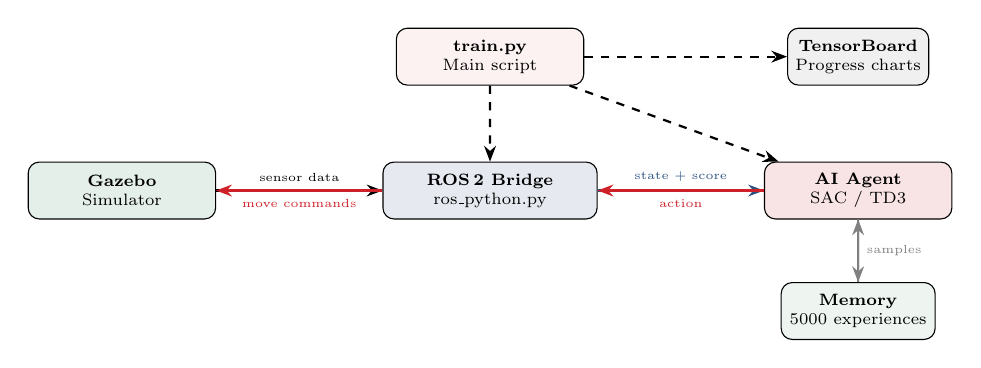
\begin{tikzpicture}[
    scale=0.85, transform shape,
    arr/.style={-{Stealth[length=2mm]}, thick},
    lbl/.style={font=\tiny, midway},
    box/.style={draw, rounded corners, minimum height=0.85cm,
                align=center, font=\scriptsize}
  ]
    \node[box, fill=softgreen!12, minimum width=2.8cm]
      (gz) at (0, 0) {\textbf{Gazebo}\\Simulator};
    \node[box, fill=softblue!12, minimum width=3.2cm]
      (ros) at (5.5, 0) {\textbf{ROS\,2 Bridge}\\ros\_python.py};
    \node[box, fill=upecred!12, minimum width=2.8cm]
      (drl) at (11, 0) {\textbf{AI Agent}\\SAC / TD3};
    \node[box, fill=softgreen!8, minimum width=2.3cm]
      (buf) at (11, -1.8) {\textbf{Memory}\\5000 experiences};
    \node[box, fill=upecred!6, minimum width=2.8cm]
      (train) at (5.5, 2.0) {\textbf{train.py}\\Main script};
    \node[box, fill=gray!12, minimum width=2.0cm]
      (tb) at (11, 2.0) {\textbf{TensorBoard}\\Progress charts};

    \draw[arr] (gz) -- node[above, lbl] {sensor data} (ros);
    \draw[arr, upecred] (ros) -- node[below, lbl] {move commands} (gz);
    \draw[arr, softblue] (ros) -- node[above, lbl] {state + score} (drl);
    \draw[arr, upecred] (drl) -- node[below, lbl] {action} (ros);
    \draw[arr, gray] (drl) -- (buf);
    \draw[arr, gray] (buf) -- node[right, lbl] {samples} (drl);
    \draw[arr, dashed] (train) -- (ros);
    \draw[arr, dashed] (train) -- (drl);
    \draw[arr, dashed] (train) -- (tb);
  \end{tikzpicture}
  \end{center}

  \vspace{0.2em}

  \begin{center}
    {\small
    \textbf{Gazebo} simulates the world $\rightarrow$
    \textbf{ROS\,2} delivers the data $\rightarrow$
    \textbf{AI} decides how to move $\rightarrow$
    \textbf{Memory} stores experience for later learning}
  \end{center}
\end{frame}

% ============================================================
\section{Results}
% ============================================================

% -------------------- SLIDE: Evaluation --------------------
\begin{frame}{How We Measure Progress}

  \begin{columns}[T]
    \begin{column}{0.48\textwidth}
      \small
      After every training round, the robot is tested on
      \textbf{10 fixed scenarios} (same obstacles, same goals)
      to track improvement fairly.

      \vspace{0.4em}
      \textbf{What we track (via TensorBoard):}
      \begin{itemize}\small
        \item \textbf{Goal rate}: how often it reaches the goal
        \item \textbf{Collision rate}: how often it crashes
        \item \textbf{Average reward}: overall performance score
      \end{itemize}
    \end{column}

    \begin{column}{0.48\textwidth}
      \centering
      \textbf{Expected training progress:}

      \vspace{0.3em}
      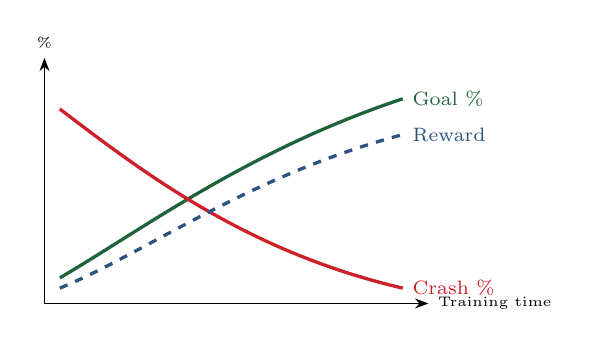
\begin{tikzpicture}[scale=0.65]
        \draw[-{Stealth}] (0,0) -- (7.5,0) node[right, font=\tiny] {Training time};
        \draw[-{Stealth}] (0,0) -- (0,4.8) node[above, font=\tiny] {\%};

        \draw[very thick, softgreen!80!black]
          (0.3, 0.5) .. controls (2, 1.5) and (4, 3.0) .. (7, 4.0);
        \node[font=\scriptsize, softgreen!80!black, right] at (7, 4.0)
          {Goal \%};

        \draw[very thick, upecred]
          (0.3, 3.8) .. controls (2, 2.5) and (4, 1.0) .. (7, 0.3);
        \node[font=\scriptsize, upecred, right] at (7, 0.3)
          {Crash \%};

        \draw[very thick, softblue, dashed]
          (0.3, 0.3) .. controls (2, 1.0) and (4, 2.5) .. (7, 3.3);
        \node[font=\scriptsize, softblue, right] at (7, 3.3)
          {Reward};
      \end{tikzpicture}

      \vspace{0.3em}
      \small
      As training goes on: goals $\uparrow$, crashes $\downarrow$,
      reward $\uparrow$. This proves the robot is learning!
    \end{column}
  \end{columns}
\end{frame}

% -------------------- SLIDE: AI vs Traditional --------------------
\begin{frame}{AI Navigation vs.\ Traditional Methods}

  \begin{columns}[T]
    \begin{column}{0.48\textwidth}
      \begin{block}{Traditional methods}
        \begin{itemize}\small
          \item Need a \textbf{map first} (built with SLAM)
          \item Many separate pieces to configure
          \item Settings tuned \textbf{by hand}
          \item Predictable but rigid
          \item Bad with \textbf{moving obstacles}
        \end{itemize}
      \end{block}
    \end{column}
    \begin{column}{0.48\textwidth}
      \begin{exampleblock}{Our AI approach}
        \begin{itemize}\small
          \item \textbf{No map needed} -- uses live laser data
          \item One single network does everything
          \item Learns \textbf{on its own} from practice
          \item Adapts to new situations
          \item Handles \textbf{moving obstacles} naturally
        \end{itemize}
      \end{exampleblock}
    \end{column}
  \end{columns}

  \vspace{0.3em}

  \begin{alertblock}{Key takeaway}
    \small The neural network \textbf{replaces the entire traditional
    planning system}. It reads sensor data and outputs movement commands
    directly -- all in less than 1 millisecond.
  \end{alertblock}
\end{frame}

% -------------------- SLIDE: Pros/Cons --------------------
\begin{frame}{Strengths and Limitations}

  \begin{columns}[T]
    \begin{column}{0.48\textwidth}
      \textbf{\color{softgreen!80!black}What works well:}
      \begin{itemize}\small
        \item Simple pipeline (sensor $\rightarrow$ AI $\rightarrow$ move)
        \item No manual tuning needed
        \item Handles random and moving obstacles
        \item Pre-training gives a fast start
        \item Very fast decisions ($<$1\,ms)
      \end{itemize}
    \end{column}
    \begin{column}{0.48\textwidth}
      \textbf{\color{upecred}Current limitations:}
      \begin{itemize}\small
        \item Needs a lot of training time
        \item Hard to guarantee it will never crash
        \item The AI is a ``black box'' (hard to explain)
        \item Trained in simulation -- may not work
              perfectly on a real robot
      \end{itemize}
    \end{column}
  \end{columns}

  \vspace{0.4em}

  \begin{block}{Bottom line}
    \small AI navigation is great for complex environments where
    traditional methods struggle. The main challenge is making sure
    the AI is \textbf{safe and reliable} enough for real-world use.
  \end{block}
\end{frame}

% ============================================================
\section{Demo}
% ============================================================

% -------------------- SLIDE: How to Run --------------------
\begin{frame}[fragile]{Running the Project}

  \textbf{Step 1:} Set up the environment (in each terminal)
  \begin{lstlisting}[language=bash]
export DRLNAV_BASE_PATH=~/DRL-Robot-Navigation-ROS2
export TURTLEBOT3_MODEL=waffle
source /opt/ros/foxy/setup.bash
source $DRLNAV_BASE_PATH/install/setup.bash
  \end{lstlisting}

  \textbf{Step 2:} Start the simulator (Terminal 1)
  \begin{lstlisting}[language=bash]
ros2 launch turtlebot3_gazebo ros2_drl.launch.py
  \end{lstlisting}

  \textbf{Step 3:} Start training the AI (Terminal 2)
  \begin{lstlisting}[language=bash]
python3 src/drl_navigation_ros2/train.py
  \end{lstlisting}

  \textbf{Step 4:} Watch the progress (Terminal 3)
  \begin{lstlisting}[language=bash]
tensorboard --logdir runs   # open http://localhost:6006
  \end{lstlisting}
\end{frame}

% ============================================================
\section{Conclusion}
% ============================================================

% -------------------- SLIDE: Conclusion --------------------
\begin{frame}{Conclusion}
  \small
  \begin{enumerate}
    \setlength{\itemsep}{0.3em}
    \item We built a system where a robot \textbf{learns to navigate
          on its own} using AI (Deep Reinforcement Learning)
    \item It uses only \textbf{laser sensor data} -- no map needed
    \item The AI (\textbf{SAC algorithm}) learns through trial and error
          in a simulated world (\textbf{Gazebo})
    \item \textbf{Pre-training} from expert data gives a head start;
          \textbf{progressive difficulty} ensures stable learning
    \item \textbf{ROS\,2} connects the AI to the simulator seamlessly
    \item We tracked progress using \textbf{TensorBoard}: goal rate
          goes up, collision rate goes down
  \end{enumerate}

  \vspace{0.3em}

  \begin{exampleblock}{Mission accomplished}
    \small We showed how an \textbf{AI-based navigation approach} can be
    integrated into a ROS robot system, replacing traditional planning
    with a neural network that learns from experience.
  \end{exampleblock}
\end{frame}

% -------------------- SLIDE: Thank You --------------------
{
\setbeamertemplate{footline}{}
\begin{frame}
  \centering
  \vspace{0.8cm}

  
\includegraphics[height=1.5cm]{figures/UPEC-logo.svg.png}

  \vspace{0.6cm}
  {\Huge\bfseries\color{upecdark} Thank You}

  \vspace{0.4cm}
  {\Large\color{upecred} Questions?}

  \vspace{0.6cm}
  {\small\color{upecgray}
  \begin{tabular}{rl}
    \textbf{Authors:} & Benhamlaoui Abderrahmene Amar \& Brahimi Redha Wassim\\
    \textbf{Supervisor:} & Prof.\ Samer Mohammed\\
    \textbf{Module:} & Robotics and AI -- Master IA2S\\
    \textbf{University:} & UPEC -- Universit\'{e} Paris-Est Cr\'{e}teil\\
  \end{tabular}}

  \vspace{0.5cm}
  \textcolor{upecred}{\rule{0.5\textwidth}{1.5pt}}

  \vspace{0.2cm}
  {\footnotesize\color{upecgray}
  ROS\,2 Foxy $\cdot$ Gazebo 11 $\cdot$ SAC / TD3 $\cdot$
  TurtleBot3 $\cdot$ PyTorch}
\end{frame}
}

\end{document}
